\documentclass[a4paper]{article}

\usepackage[utf8x]{inputenc}
\usepackage[british,UKenglish]{babel}
\usepackage{amsmath}
%\usepackage{titlesec}
\usepackage{color}
\usepackage{graphicx}
\usepackage{fancyref}
\usepackage{hyperref}
\usepackage{float}
\usepackage{scrextend}
\usepackage{setspace}
\usepackage{xargs}
\usepackage{multicol}
\usepackage{nameref}
\usepackage[pdftex,dvipsnames]{xcolor}
\usepackage{sectsty}

\graphicspath{ {images/} }
\newcommand\tab[1][1cm]{\hspace*{#1}}
\hypersetup{colorlinks=true, linkcolor=black}
\interfootnotelinepenalty=10000
%\titleformat*{\subsubsection}{\large\bfseries}
\subsubsectionfont{\large}
\subsectionfont{\Large}
\sectionfont{\LARGE}
\definecolor{cleanOrange}{HTML}{D14D00}
\definecolor{cleanYellow}{HTML}{FFFF99}
\definecolor{cleanBlue}{HTML}{3d0099}
%\newcommand{\cleancode}[1]{\begin{addmargin}[3em]{3em}\fcolorbox{cleanOrange}{cleanYellow}{\texttt{\textcolor{cleanOrange}{#1}}}\end{addmargin}}
\newcommand{\cleancode}[1]{\begin{addmargin}[3em]{3em}\texttt{\textcolor{cleanOrange}{#1}}\end{addmargin}}
\newcommand{\cleanstyle}[1]{\text{\textcolor{cleanOrange}{\texttt{#1}}}}


\usepackage[colorinlistoftodos,prependcaption,textsize=footnotesize]{todonotes}
\newcommandx{\commred}[2][1=]{\textcolor{Red}
{\todo[linecolor=red,backgroundcolor=red!25,bordercolor=red,#1]{#2}}}
\newcommandx{\commblue}[2][1=]{\textcolor{Blue}
{\todo[linecolor=blue,backgroundcolor=blue!25,bordercolor=blue,#1]{#2}}}
\newcommandx{\commgreen}[2][1=]{\textcolor{OliveGreen}{\todo[linecolor=OliveGreen,backgroundcolor=OliveGreen!25,bordercolor=OliveGreen,#1]{#2}}}
\newcommandx{\commpurp}[2][1=]{\textcolor{Plum}{\todo[linecolor=Plum,backgroundcolor=Plum!25,bordercolor=Plum,#1]{#2}}}


%-----------------------------------------BEGIN DOC----------------------------------------

\begin{document}

\title{{\Huge ercesiMIPS Lab Manual{\large\linebreak\\}}{\Large A guide to Single Cyclic CPU with 7-9(11) MIPS Instructions\linebreak\linebreak}
\linebreak{\Large[\nameref{c}]}
\linebreak{\small click on it\linebreak}}
\author{\\Authors: Jianfeng An, Meng Zhang \& Danghui Wang\\\\
CS 11007 Computer Organization and Architecture\\
(Spring, 2017)\\\\
Northwestern Polytechnical University, China\\
Faculty of Computer Science\\
ERCESI}
\date{27 April 2017}
\maketitle
\newpage

%-----------------------------------------ABSTRACT-------------------------------------

{\large\bf{"SWEET JEZUS WHY!?"\\}}
\begin{addmargin}[2em]{2em}{\setstretch{0.6}{\small\textit{If you're reading this, chances are that either your arms are suffering from anemia in waiting for the TA's to finish helping the 20 people in the room, or you're trying to design in Chisel without any TA's whatsoever, and you just wanna end it all. Fret not! This document serves as a specification for basic explanations of single cyclic MIPS CPU with 7-11 instructions supporting, also a helpful links and forbidden deigning secrets whose names none dare speak.}}}
\end{addmargin}
\tableofcontents\label{c}
\newpage

%------------------------------------------TEXT--------------------------------------------

%----------------------------------------OVERVIEW-----------------------------------------

\section{Overview} \label{overview}%------------------------------
The structure of Single cyclic MIPS CPU has been introduced in CS 11007 class lecture.
\begin{itemize}
	\item{\textbf{Supported Instructions} includes \emph{sub, add, or, ori, lw, sw, lst, beq, j}, or adding \emph{addi, and, andi} for better programming experience in assembly. All these instructions can be supported without exception detecting (overflow detecting)}
    \item{\textbf{All instructions work in one cycle.} For the very beginning stage, Single Cyclic CPU model is a great example to explain how CPU works.}
    \item{\textbf{Consisted of Data Path, Control Unit and Memory Unit.} To illustrate the typical systematic idea of computer, we recommend you design your first CPU with two separated modules, CPath and DPath, in such coding style, both blocks can also be easily verified separately. Additionally, if more complement MIPS ISA is chosen, this structure will be high efficient to be extended.}
    \item{\textbf{Chisel3 is also recommended.} Chisel is a powerful structural hardware description language, with more efficient expression for block, operation, and IO bundles compared with Verilog. However, the most significant feature of Chisel is that it can express the structure of system without detailed circuits coding. Further more, we prefer Chisel3 instead of Chisel2, which relies on verilator for verilog simulations instead of Synopsys vcs. The difference between these tow versions can be referenced here: \url{https://github.com/ucb-bar/chisel3/wiki/Chisel3-vs-Chisel2}.}
\end{itemize}

%-----------------------------------------Specification-------------------------------------------

\newpage
\section{Specification} \label{Specification}%------------------------------
A typical single cyclic CPU core is consisted of Control Unit and Data Path unit. In lecture 10~11, the whole system is illustrated in Fig. \ref{fig:singleblock}. 
\begin{figure}[ht]
 \centering
 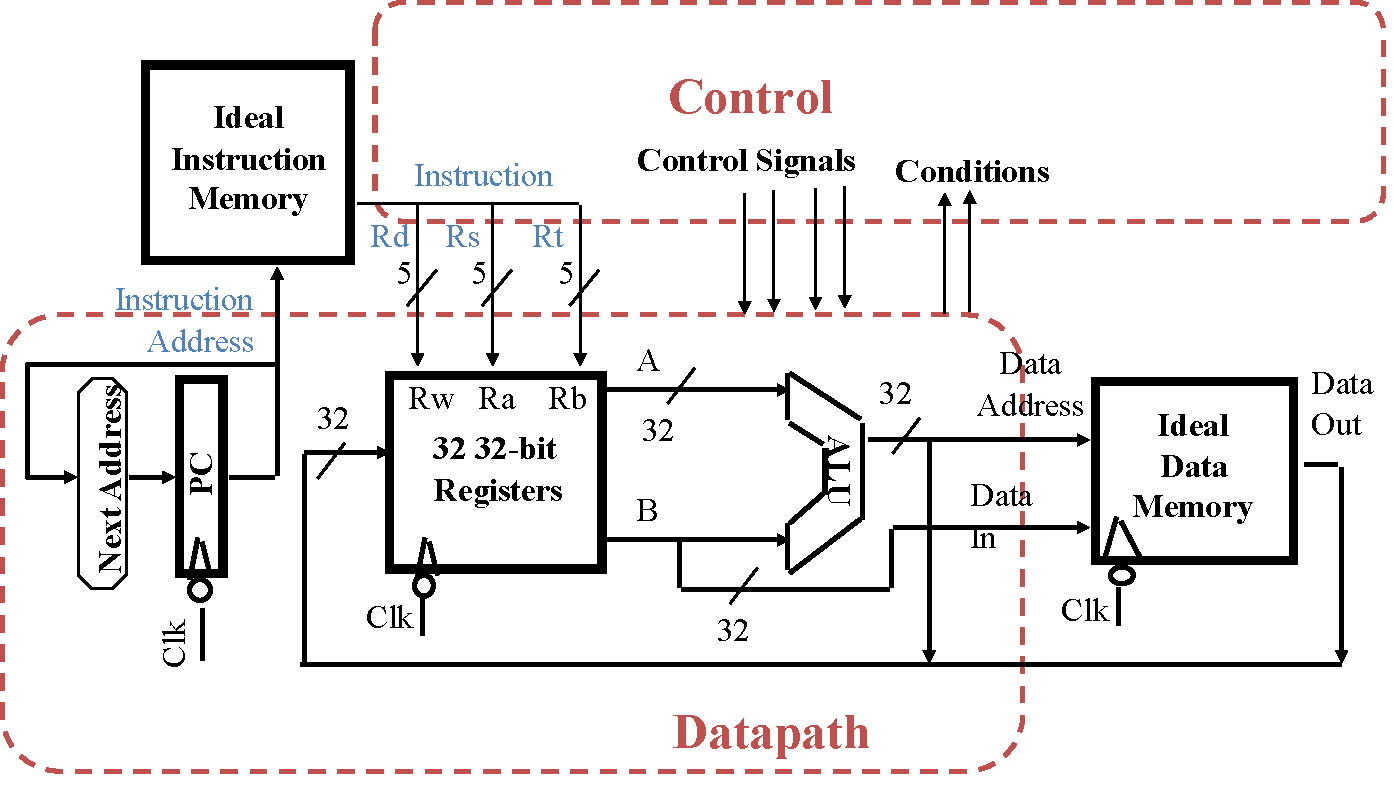
\includegraphics[height=5cm]{images/l1sys.pdf}
 \caption{Single Cyclic CPU Block Diagram}
 \label{fig:singleblock}
\end{figure}

\textbf{Two Module classes are recommended for Control Unit and Data Path Unit respectively}, as shown in following Fig. \ref{fig:modules}. Although the Harvard structure is adopted now to simplify the memory control and initialization, a MIPS adaptive memory model (Princeton Structure) is mandatory in further MIPS program test (for Multi-cyclic CPU Lab).  
\begin{figure}[ht]
 \centering
 \includegraphics[height=7cm]{images/l1modules.pdf}
 \caption{Single Cyclic CPU Block Diagram}
 \label{fig:modules}
\end{figure}
In Fig. \ref{fig:modules}, almost all signals can be renamed by your self except those evaluation required singles specified in Section \ref{sub:signal}.
%---------------------------------------Chisel 3------------------------------------------

\newpage
\section{Chisel3 101} \label{Datatypes}%------------------------------
TBD
 
%---------------------------------------Evalu Req------------------------------------------

\newpage
\section{Evaluation Requirement} \label{sec:Functions}%------------------------------
\subsection{Signal Requirement}\label{sub:signal}
TBD
%\url{}


\end{document}

